\subsection{Matrices Handling Changes} \label{ssec:val_matrices}

    \begin{figure}[ht]
        \centering
        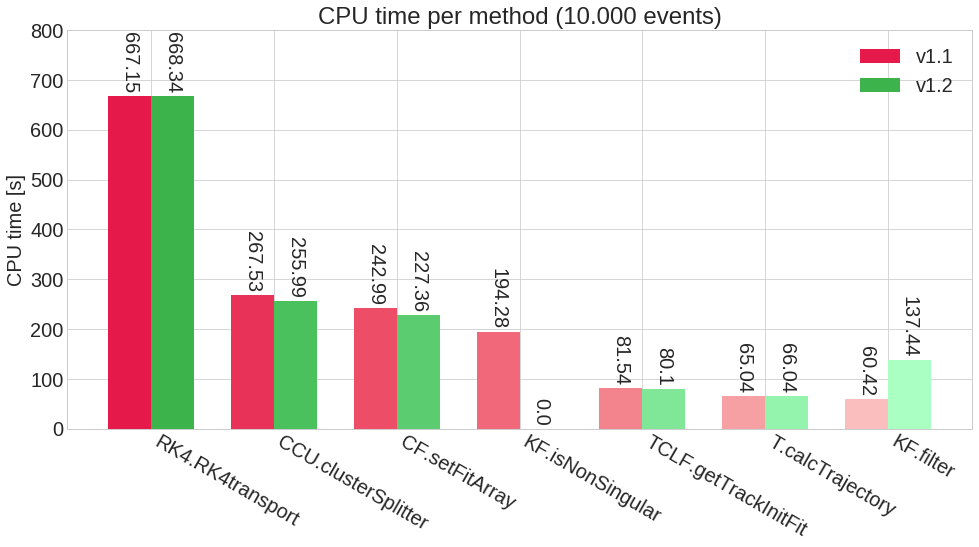
\includegraphics[scale=0.44]{methods_times/1_2}
        \caption{\label{fig:methods_times-1_2} Method CPU times, version $1.2$ compared with $1.1$.}
    \end{figure}

The changes described in Section \ref{ssec:prop_matrices} improve the total CPU time per event of DCHB and DCTB by $4.2\%$ (from $118.14$ to $113.19$ [ms]) and by $3.2\%$ (from $44.34$ to $42.93$ [ms]) respectively.
As shown in Figure \ref{fig:methods_times-1_2}, the \texttt{isNonSingular} method sees a reduction down to $0$ [s] while the \texttt{filter} method sees a significant increase of $127.5\%$ ($77.04$ [s]) and the rest of the methods see very little change, which is only attributed to error between measurements.

The increased time in the \texttt{filter} method is attributed to the fact that the time that was taken by the \texttt{isNonSingular} method is transferred to it due to the changes made to the code. % Note: I sincerely have no idea on to how this happened, I'm guessing it's one of those weird java things.
The net gain in time is of $46.0\%$ (from $254.70$ to $137.44$ [s] in total), which isn't great when considering that the total reduction seen in DCHB and DCTB's times is only of $6.36$ [ms] per event.

The contrast between all the work done and the unremarkable change is attributed to the fact that this work is focused on finely optimizing the code and finding the best methods available to solve the problems, which goes against the principles behind the Java HotSpot compiler as it favors simple-to-understand methods and optimizes them while the application is running, neglecting already optimized code~\cite{meloan1999java}.
This is opposite to the normal behaviour of more standard compilers like gcc, which in turn favors well-optimized code. % Note: Perhaps this last statement needs a citation.

